\documentclass[a4paper, article, oneside, USenglish, IN5460]{memoir}

%% Title page
\usepackage{style/projectfp} 


%% Encoding
\usepackage[utf8]{inputenx} % Source code
\usepackage[T1]{fontenc}    % PDF
\usepackage{float}


%% Fonts and typography
\usepackage{lmodern}           % Latin Modern Roman
\usepackage[scaled]{beramono}  % Bera Mono (Bitstream Vera Sans Mono)
\renewcommand{\sfdefault}{phv} % Helvetica
\usepackage[final]{microtype}  % Improved typography
\renewcommand{\abstractnamefont}{\sffamily\bfseries}                 % Abstract
\renewcommand*{\chaptitlefont}{\Large\bfseries\sffamily\raggedright} % Chapter
\setsecheadstyle{\large\bfseries\sffamily\raggedright}               % Section
\setsubsecheadstyle{\large\bfseries\sffamily\raggedright}            % Subsection
%%\setsubsubsecheadstyle{\normalsize\bfseries\sffamily\raggedright}    % Subsubsection
\setparaheadstyle{\normalsize\bfseries\sffamily\raggedright}         % Paragraph
\setsubparaheadstyle{\normalsize\bfseries\sffamily\raggedright}      % Subparagraph

%% Mathematics
\usepackage{amssymb}   % Extra symbols
\usepackage{amsthm}    % Theorem-like environments
\usepackage{thmtools}  % Theorem-like environments
\usepackage{mathtools} % Fonts and environments for mathematical formuale
\usepackage{mathrsfs}  % Script font with \mathscr{}
% Bibliography
\usepackage[backend=biber,style=numeric-comp]{biblatex}

% Plotting
\usepackage[utf8]{inputenc}
\usepackage{pgfplots}
\DeclareUnicodeCharacter{2212}{−}
\usepgfplotslibrary{groupplots,dateplot}
\usetikzlibrary{patterns,shapes.arrows}
\pgfplotsset{compat=newest}


\usepackage{graphicx}
\usepackage{subcaption}
\usepackage{mwe}

\newlength\figH
\newlength\figW
\setlength{\figH}{8cm}
\setlength{\figW}{12cm}


\DeclareMathOperator*{\min}{\text{\Large minimize}}

\usepackage{optidef}
\usepackage{listings} 


\title{ Wind Energy Forecasting }
\authors{W. Cai, F. Ofstad, E. F. Rørstad}

\addbibresource{bibliography.bib}

\begin{document}

\shorthandoff{}

\projectfrontpage


\chapter*{Introduction}
\subsection{linear regression for wind power prediction}
the linear model is defined as $y=wx+b$.
And the residual for observation $i$ is $e_i =y_i -(wx_i+b)$. Thus, linear regression is used to minimize the sum of residual squares, shown as followed:
\begin{equation}
\begin{aligned}
\min_{w,b}\sum_{i=1}^{n} [y_i-(wx_i+b)]^2
\end{aligned}
\end{equation}
\newline


\subsection{K-NN for wind power prediction}
We Calculate the distance between $x$ and each training data point $x_i$ and select $k$ data points with the smallest distances to $x$, and compute the average (or weighted average) of the target values $y_{ij}$ of these $k$ data points to 
$x$ :
\begin{equation}
\begin{aligned}
\Bar{y} = \sum_{j=1}^{k} w_{ij}\frac{y_{ij}}{k}
\end{aligned}
\end{equation}
\newline

\subsection{SVR for wind power prediction}
We use a hyperplane to show the 
relationship between input features ( wind speed and wind direction for example) and the wind power generated. The goal of SVR is to find a function that maximize the width of $\epsilon$-tube, and also minimize the errors of all points outside the tube.
We use a soft SVR with small tolerance (0.1) to manage our model fitting

\newline


\subsection{ANN for wind power prediction}
Each single artificial neuron is defined as the following: 
\begin{equation}
\begin{aligned}
y(x) = f(\sum_{i=1}^{n} w_i*x_i)
\end{aligned}
\end{equation}
where $y(x)$ is the variable for output signal, $x_i$ are variables for input signals, $w_i$ are the weights of corresponding input signals. $f()$ is the activation function of each node. Hidden layers with hidden nodes in between of inputs and the output forms a neural network topology
\newline

\subsection{RNN  for wind power prediction}
We have the present input $x_t$,  the hidden state $h_t$ and three weights: U for the input layer, W for the hidden layer and V for the output layer.Time recurrence is introduced with $h_t$ and its previous state $h_{t-1}$. 

\begin{figure}[H]
\centering
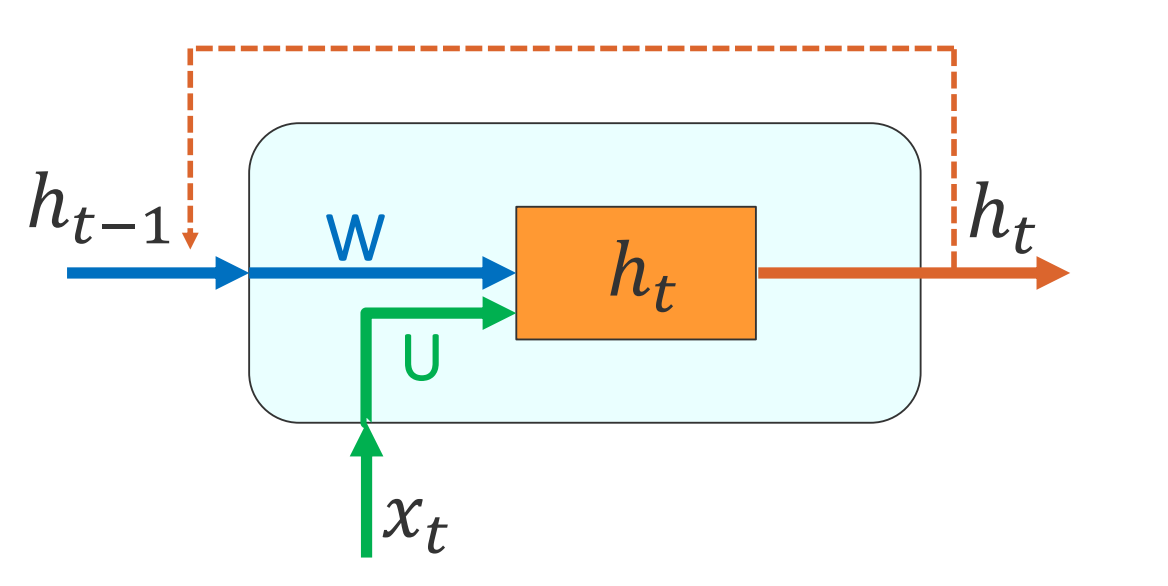
\includegraphics[width=0.8\linewidth]{fig/rnn.png}
\caption{\label{fig:q41} RNN Architecture}
\end{figure}

\begin{equation}
\begin{aligned}
h_t &=f(U*x_t +W*h_{t-1})\\
y_t &= V*f(h_t)

\end{aligned}
\end{equation}
\newline
$f$ as the activation function
\chapter*{Question 1}

SVR performs the best out of the four models with an RMSE of 0.214, as seen in Table \ref{tab:q1-RMSE-comparison}  showing the RMSE value of each of the four models. The ANN is second best with an RMSE of 0.215 and LR/KNN has the same RMSE of 0.217.

\begin{table}[H]
    \centering
    \begin{tabular}{|c|c|c|c|c|} \hline 
        Method & LR & KNN & SVR & ANN\\ \hline 
        RMSE&  0.217&  0.217&  0.214& 0.215\\ \hline
    \end{tabular}
    \caption{Table of RMSE for the Four Methods}
    \label{tab:q1-RMSE-comparison}
\end{table}

Figure \ref{fig:q1-training-data} demonstrates model predictions on training data. LR, though functional, is constrained by its linear modeling capability, inaccurately predicts negative power at low wind speeds. KNN (k=1000) mirrors LR's RMSE but ensures valid outputs. SVR outperforms both ANN and KNN, even though it maintains a minimum prediction of 0.1 power output and excelling with smaller datasets through effective generalization, despite inaccuracies at low wind speeds. ANN, capable of complex modeling, is hindered by the small dataset size. Both KNN and SVR have undergone basic parameter tuning, with SVR showing superior performance and less sensitivity to outliers. LR, though functional, is constrained by its linear modeling capability.
\begin{figure}[H]
    \centering
    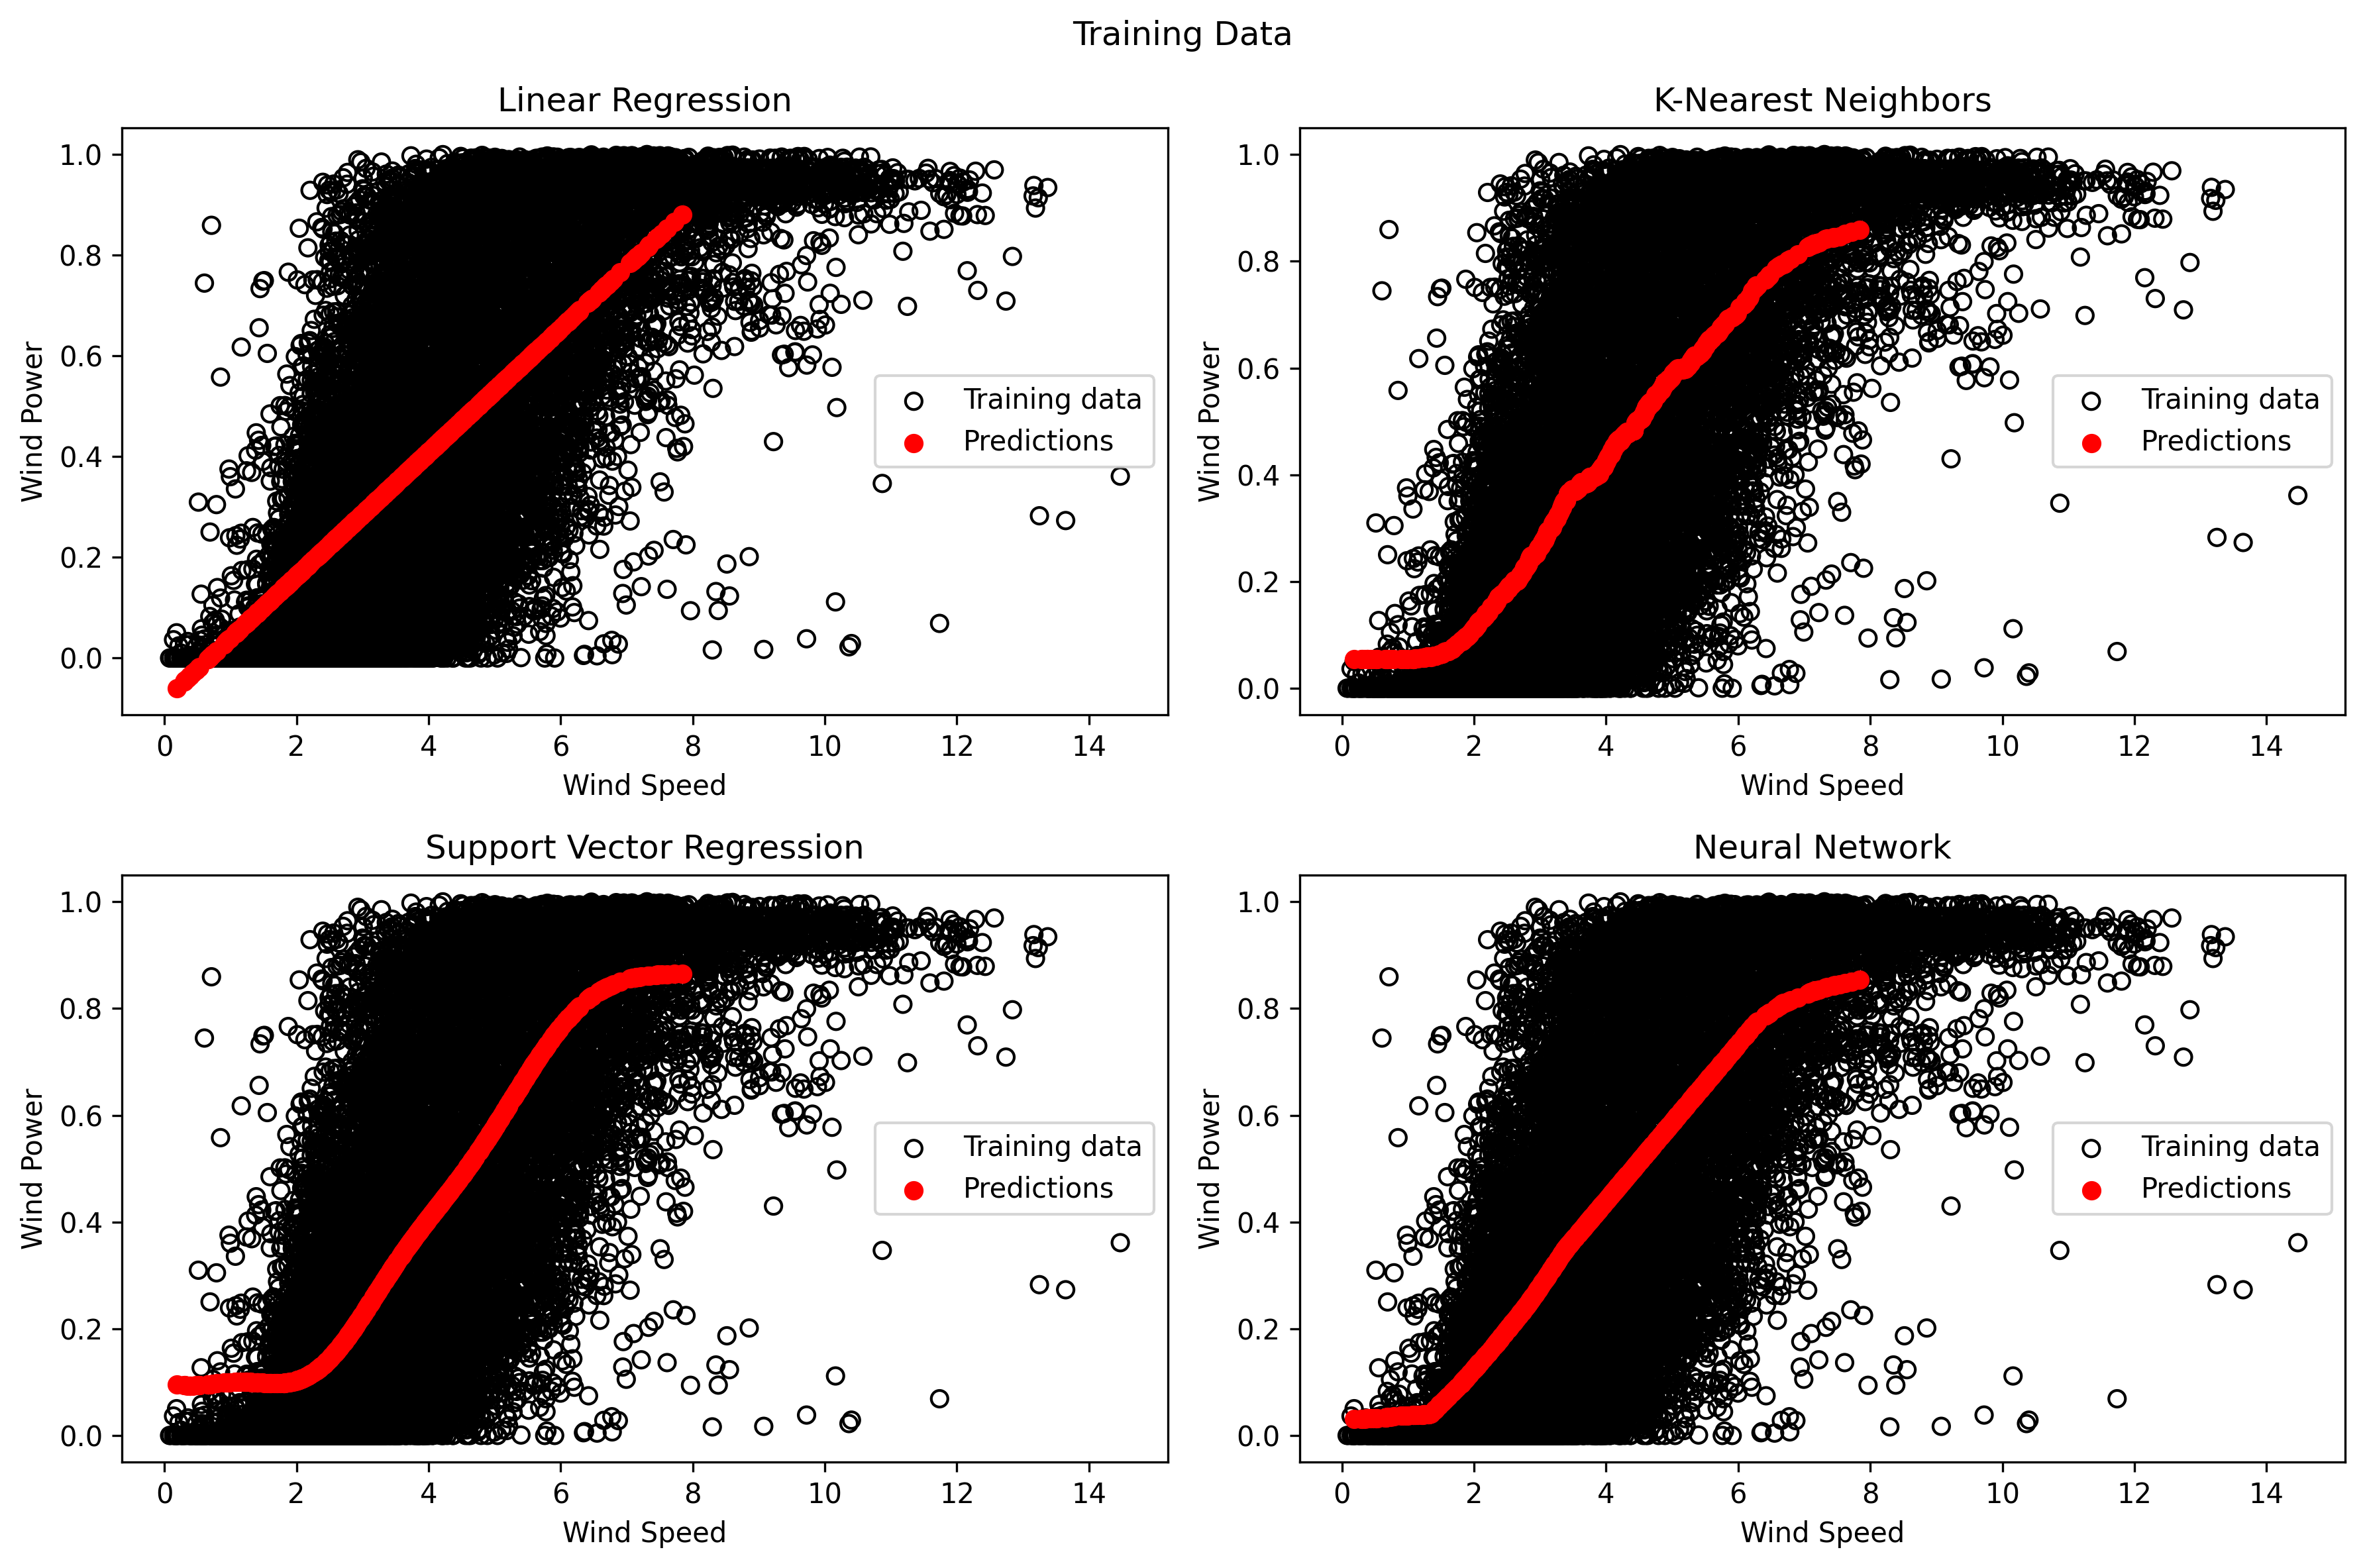
\includegraphics[width=1\linewidth]{fig/q1-ALL-training.png}
    \caption{The figure shows how each model conforms to the training data. It shows what wind power values are predicted for the given wind speed.}
    \label{fig:q1-training-data}
\end{figure}

Figure \ref{fig:q1-forecast-comparison}  shows the forecasted vs. actual power of the four models. All models performs okay, but they seem to struggle with predicting peak power. LR predicts negative power output in some places, which is wrong. SVR predicts badly for low power compared to the actual power. 
\begin{figure}[H]
    \centering
    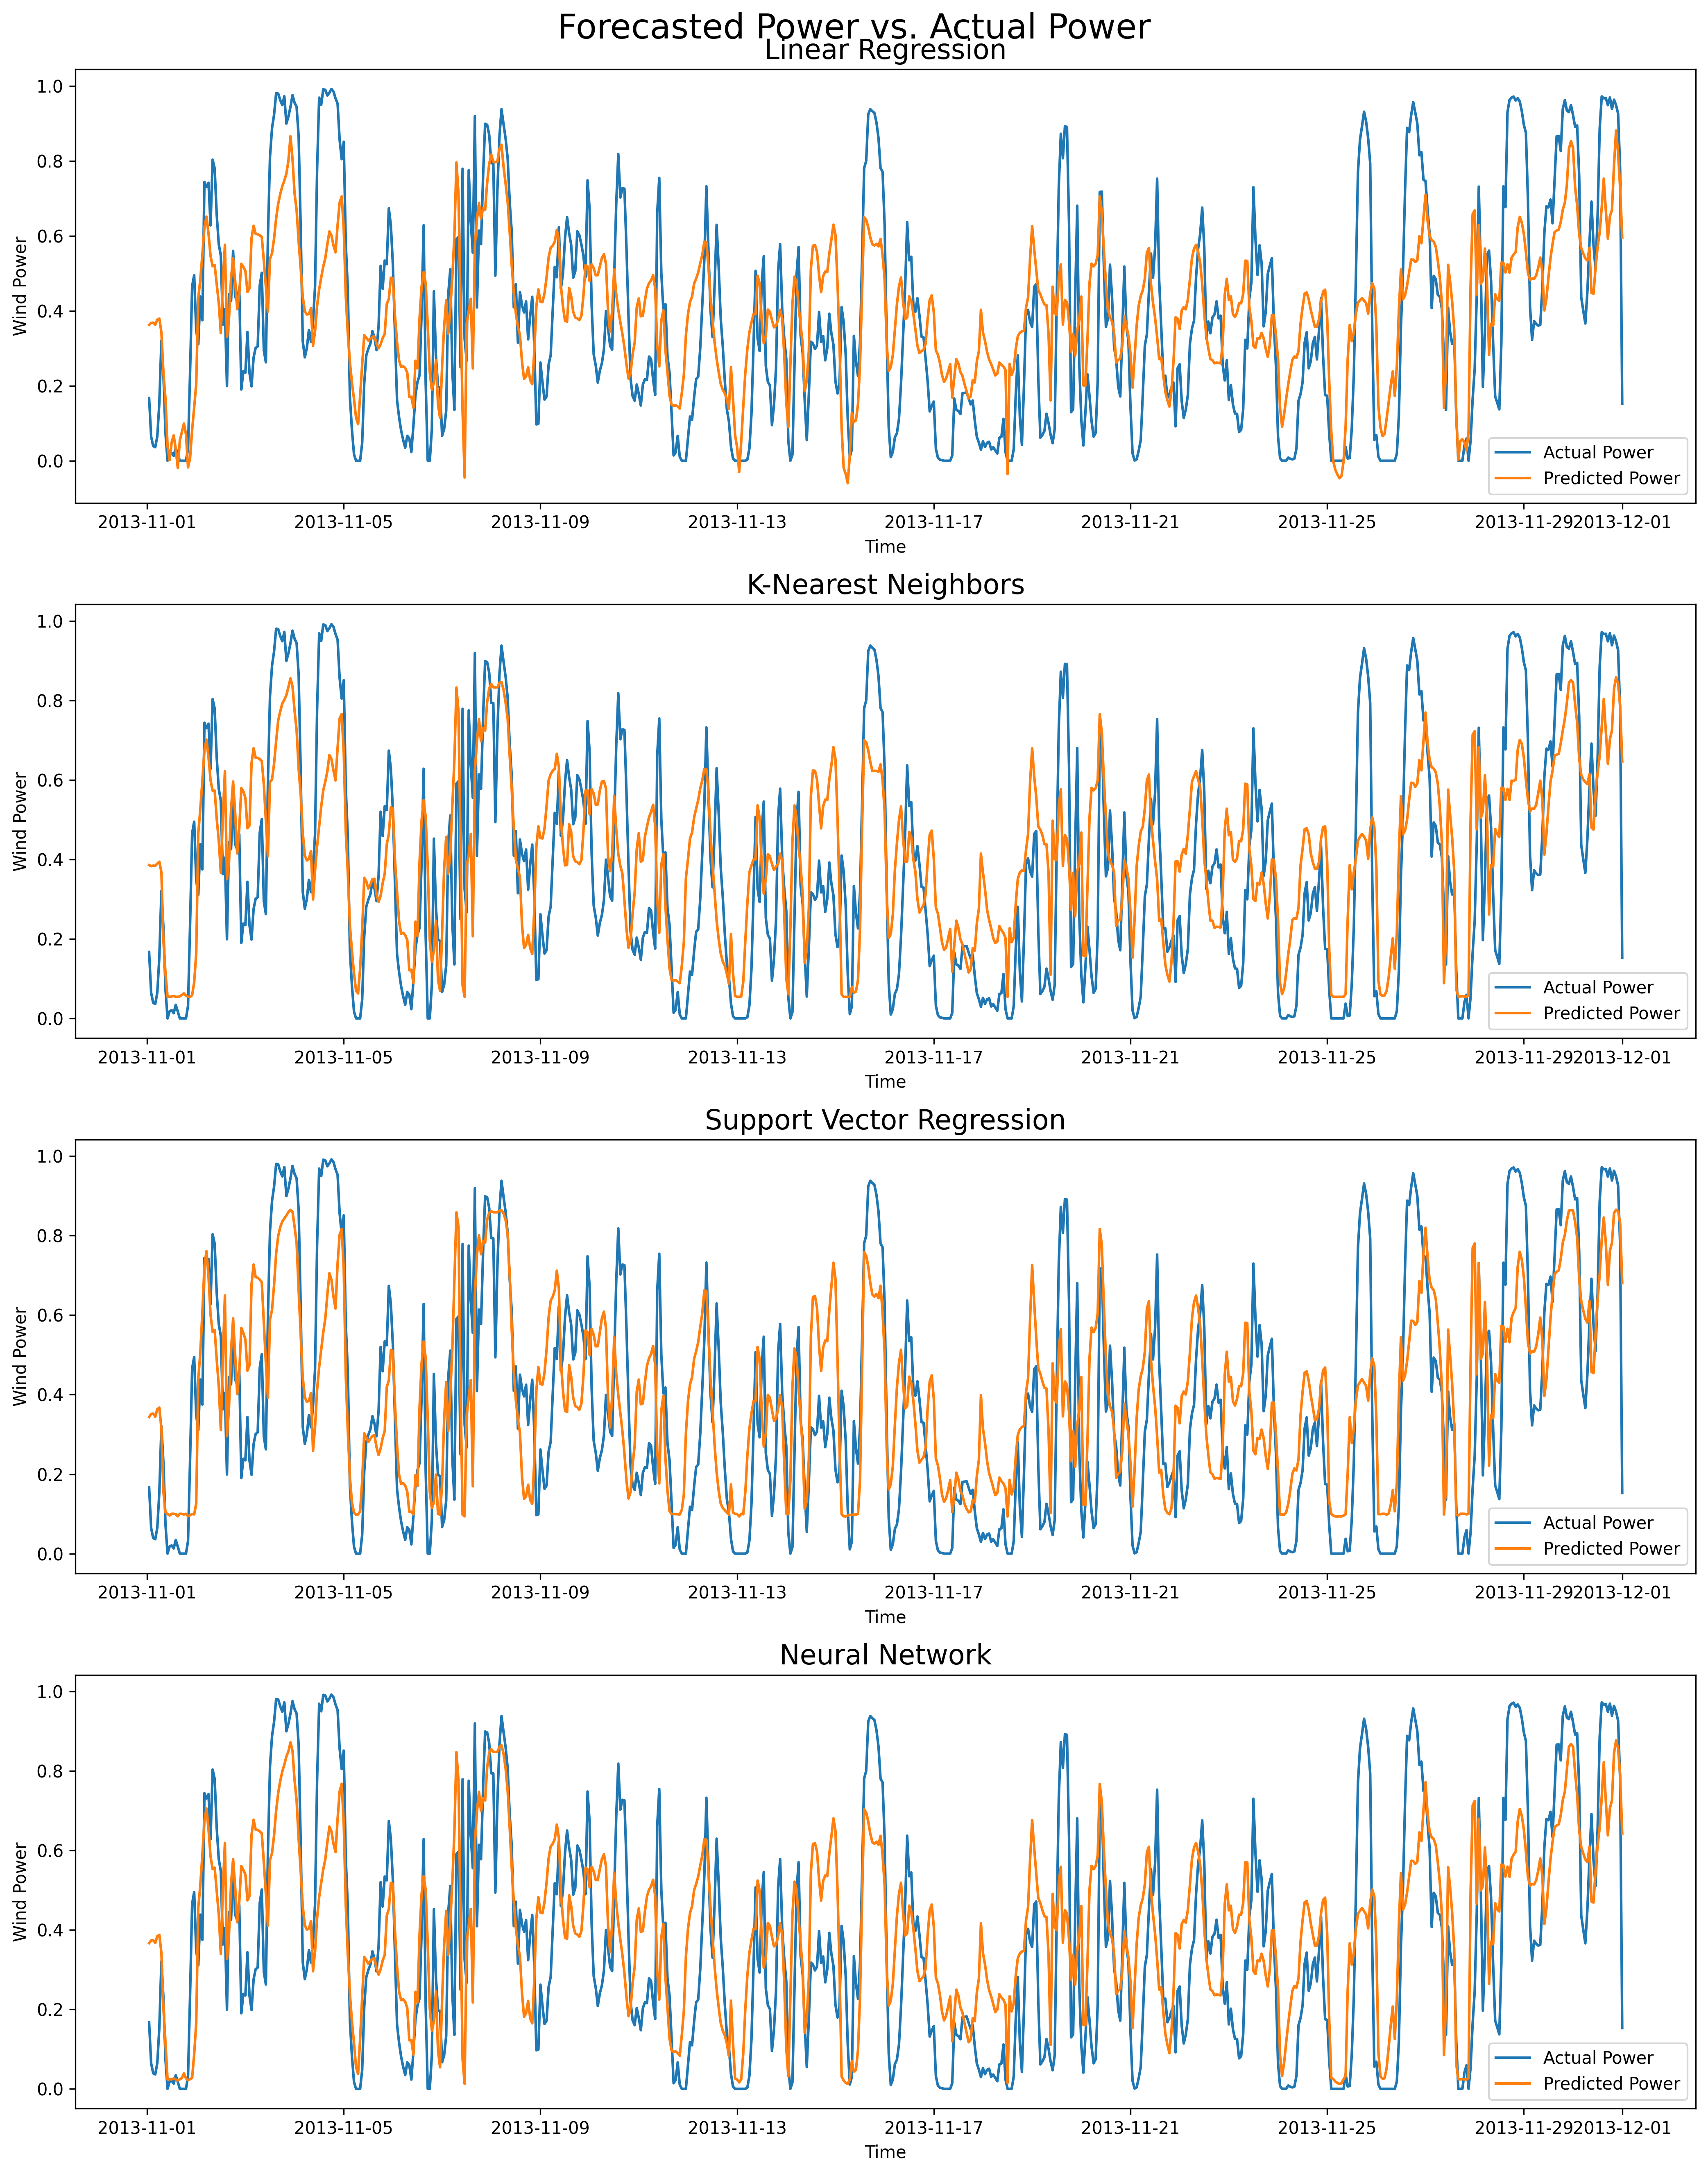
\includegraphics[width=1\linewidth]{fig/q1-ALL-forecast.png}
    \caption{Comparison of forecasts }
    \label{fig:q1-forecast-comparison}
\end{figure}


\chapter*{Question 2}

To iterate on the Linear Regression Model, we include additional variables to see what effect it has on the predictive power of the model.

From the dataset we calculate the wind direction using the zonal (v10) and meridional (u10) components using the following equation:

\begin{equation}
WindDirection = \frac{\pi}{2} - \arctan \left(\frac{v_{10}}{u_{10}}\right) \mod 2\pi
\end{equation}

We modulate the equation to ensure the value is between 0 and 1 radians.

We then update our linear model with an additional independant variable - Wind direction. Our updated model is thus:

\begin{equation}
WindPower = \beta_0 + \beta_1 \cdot WindSpeed + \beta_2 \cdot WindDirection + \epsilon
\end{equation}


Running the prediction model we get the following coefficients for the two independent variables:

\begin{table}[H]\centering
\begin{tabular}{|l|l|}
\hline
$\beta_1$ & 0.12654118  \\ \hline
$\beta_2$   & 0.01634835   \\ \hline
\end{tabular}
\end{table}

As we can see Wind Speed has the larger affect on predicting Wind power, but including Wind Direction still produces a more accurate model if only slightly.

\begin{figure}[H]
    \centering
    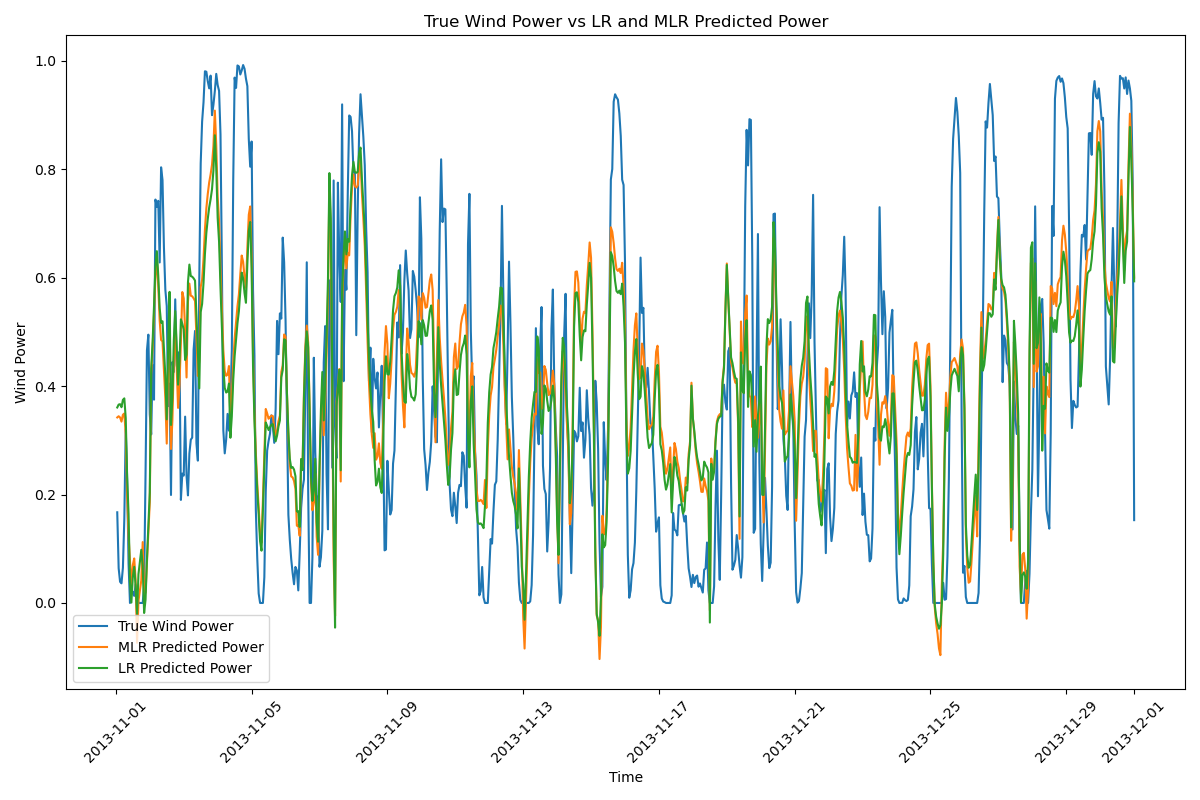
\includegraphics[width=1\linewidth]{fig/q2-forecast.png}
    \caption{Comparing LR and MLR predictions with the actual power}
    \label{fig:q2-forecast}
\end{figure}

The prediction using Multiple Linear Regression is slightly more accurate than the Linear Model, especially during days of higher variance. This is also reflected in the RMSE being slightly lower for MLR. MLR is taking more parameters into the model, which is more closely-related in a real-world scenario where wind speed is not the only factor to power generated 

\begin{table}[H]\centering
\begin{tabular}{|l|l|l|}
\hline
Method & LR & MLR  \\ \hline
RMSE   & 0.217  & 0.211    \\ \hline
\end{tabular}
\end{table}


\chapter*{Question 3}
% LR, SVR, ANN need to be time series with a window size of 1
% Please explain about how you encode the data as the input and the output in these models.
In order to forecast time-series data we first need to do some simple prepossessing of the training data. After removing all columns except for the Timestamp and Power, we now need to create a sliding window for our training data. In order to do this, we split the data up into sequences such that $x$ at time $t$ has a corresponding $y$ at time $t+1$. We thereby train the models by predicting the next value.

The Linear Regression models takes a simple approach to see if there is a linear relationship between time and power. It then uses this linear relationship to predict the power for other times.

The Artificial Neural Network takes in the same data, but will try to find weights that reflect the data instead of relying on a linear relationship. For the ANN we use a simple sequential network with a 10 node dense layer, training the model for 20 epochs.

The RNN model uses the more complicated LSTM layer, allowing it to retain (and discard) memory from previous iterations.

For all the models we've set the window size to 1.

\begin{figure}[H]
    \centering
    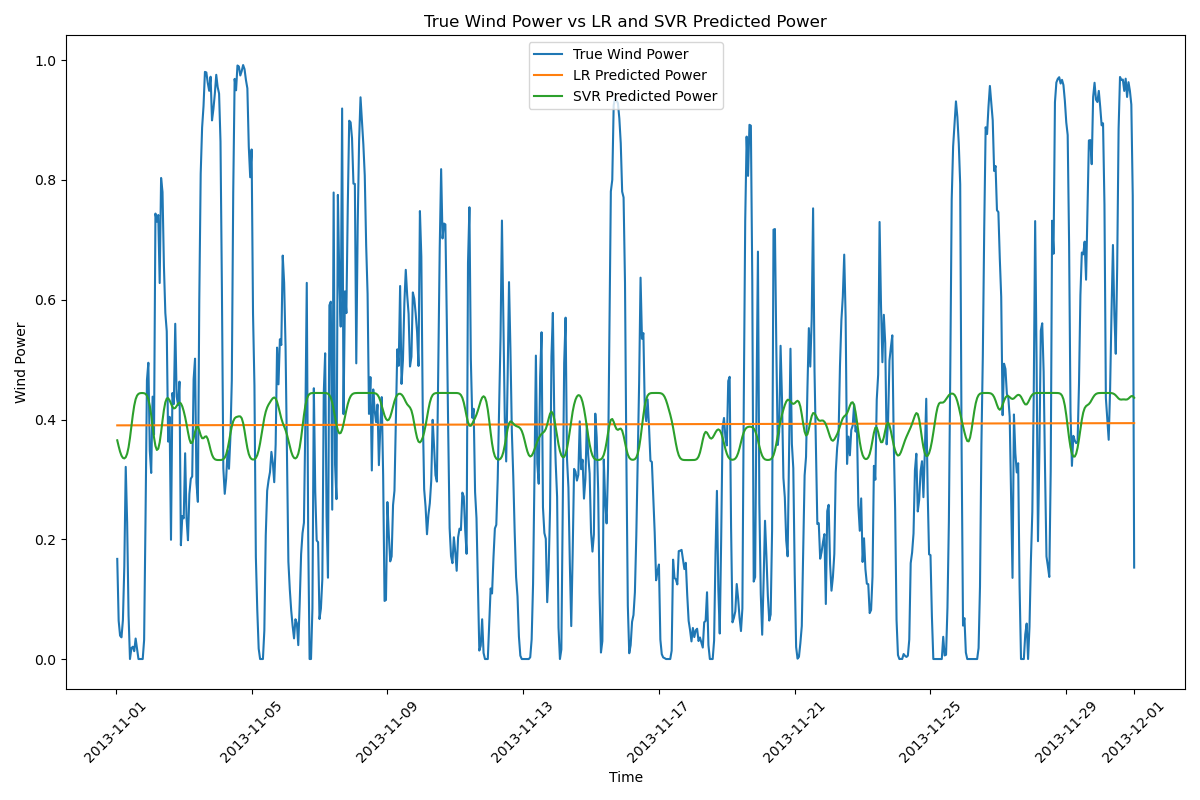
\includegraphics[width=1\linewidth]{fig/q3-LR-SVR.png}
    \caption{Comparing LR and SVR predictions with the actual power}
    \label{fig:q3-lr-svr}
\end{figure}

Graph \ref{fig:q3-lr-svr} indicates that While the models can predict the patterns, they struggle with the higher and lower values. The linear Regression models seems to outperform the SVR, which the corresponding RMSE values also confirm.


\begin{figure}[H]
    \centering
    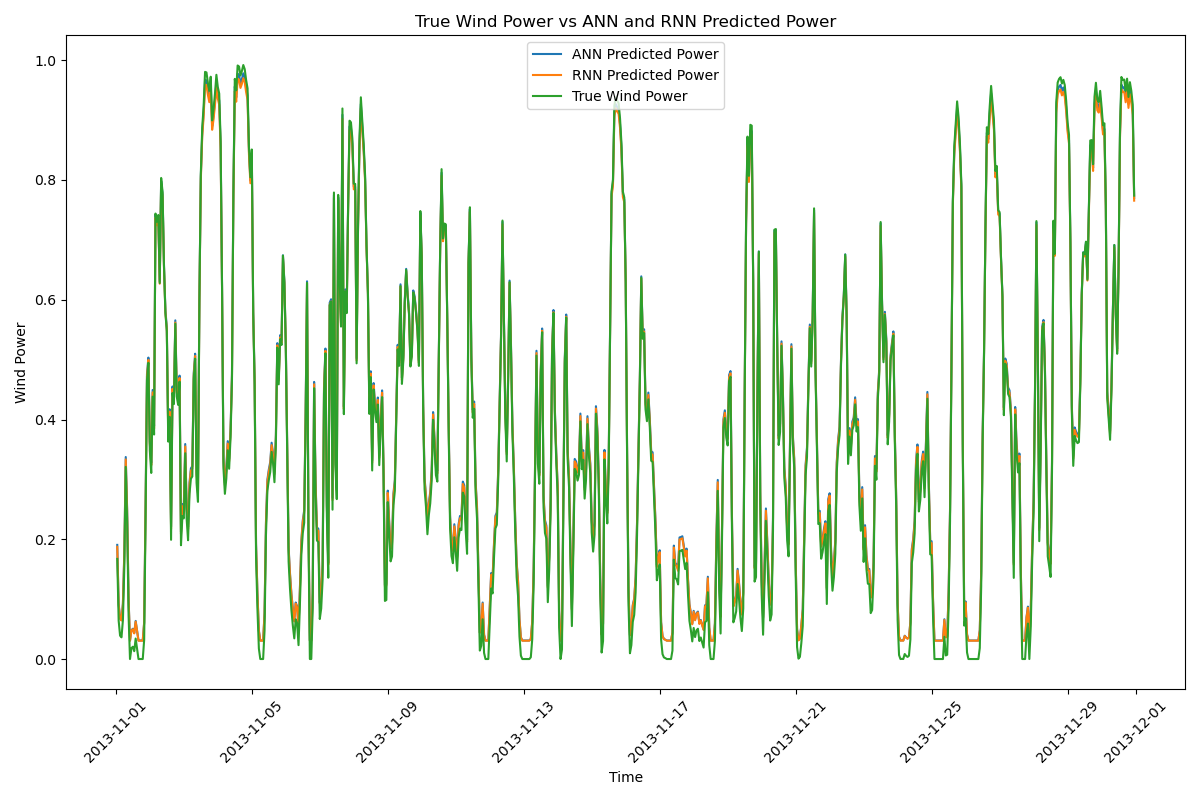
\includegraphics[width=1\linewidth]{fig/q3-ANN-RNN.png}
    \caption{Comparing ANN and RNN predictions with the actual power}
    \label{fig:q2-nn}
\end{figure}

Both Neural Networks outperform the lr and svr models, being able to more accurately predict the data. The tops are almost always reached, while some of the bottoms are still off by a certain margin.

While the RNN network provides the most accurate model, the degree to which it outperforms the others is relatively negligible considering the added complexity. This accuracy however might be more noticeable and important for larger datasets. But for smaller datasets Linear Regression is adequate while also keeping complexity to a minimum. 

\begin{table}[H]\centering
\begin{tabular}{|l|l|l|l|l|}
\hline
Method & LR     & SVR     & ANN    & RNN \\ \hline
RMSE   & 0.127  & 0.128   & 0.126      & 0.125   \\ \hline
\end{tabular}
\end{table}


\chapter*{Question 4}

\begin{figure}[H]
\centering
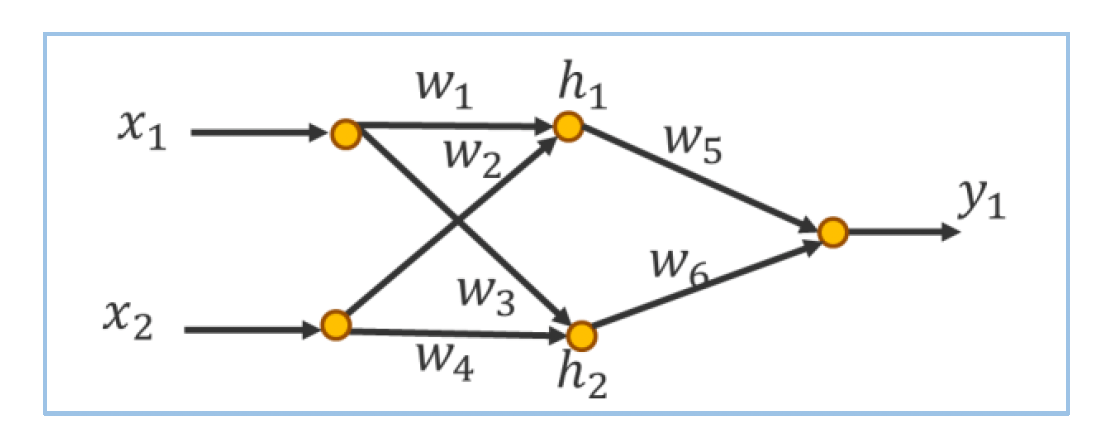
\includegraphics[width=0.8\linewidth]{fig/q4.png}
\caption{\label{fig:q4} \neural network topology}
\end{figure}
{
Given $x_1 = 0.04, x_2 = 0.2, y_1 =0.5,  \alpha = 0.4$, sigmoid activation functions
\newline
\textbf{Initial guess of weights:}
$w_1 = 0.12; 
w_2 = 0.2;
w_3 = 0.11;
w_4 = 0.25;
w_5 = 0.21;
w_6 = 0.3.$ 
% USE PYTHON SHELL TO CALCULATE!!
\newline
\textbf{ Forward: }
$\newline\text{sum}h_1 = w_1*x_1 + w_2*x_2 = 0.044800000000000006 
\newline\text{out}h_1 =sigmoid (\text{sum}h_1) =0.5111981271385566
\newline\text{sum}h_2 = w_3*x_1 + w_4*x_2 =0.054400000000000004
\newline\text{out}h_2 =sigmoid (\text{sum}h_2) =0.5135966470509216
\newline\text{sum}y_1 = w_5*\text{out}h_1 + w_6*\text{out}h_2 = 0.2614306008143733 
\newline\text{out}y_1 =sigmoid (\text{sum}y_1) = 0.5649879325949473$

\newline
\textbf{Error :}

\begin{equation}
\begin{aligned}
\text{E}_{total} &= 
\frac{1}{1}\sum(y_1 -\text{out}y_1)^2 =
0.004223431382965412

\end{aligned}
\end{equation}
\begin{equation}
\begin{aligned}
RMSE = sqrt(\text{E}_{total} ) = 0.06498793259494728
\end{aligned}
\end{equation}
\begin{equation}
\begin{aligned}
\text{E'}_{total}&= 2*(y_1 - \text{out}y_1)*(-1)= 0.12997586518989457
\end{aligned}
\end{equation}

\newline Because $\text{E'}_{total} >0 $, we use gradient descent to update $w_1 \ldots w_6 $



\newline
\textbf{Updating weights :}

for $w_6$ :
\begin{equation}
\begin{aligned}
\frac{\partial \text{E}_{total}  }{\partial w_6} &= 
\frac{\partial \text{E}_{total}}{\partial \text{out}y_1} *\frac{\partial  \text{out}y_1}{\partial \text{sum}y_1}*\frac{\partial \text{sum}y_1}{\partial  w_6}\\
&= [2*(y_1 -\text{out}y_1)*(-1)] * [\text{out}y_1(1-\text{out}y_1)] *\text{out}h_2 \\
& = 0.01640685626590058
\end{aligned}
\end{equation}


\begin{equation}
\begin{aligned}
w^+_6 &= w_6 - \alpha * \frac{\partial \text{E}_{total}  }{\partial w_6} \\
& =  0.29343725749363975
\end{aligned}
\end{equation}


\newline
for $w_5$ :
\begin{equation}
\begin{aligned}
\frac{\partial \text{E}_{total}  }{\partial w_5} &= \frac{\partial \text{E}_{total}}{\partial \text{out}y_1} *\frac{\partial  \text{out}y_1}{\partial \text{sum}y_1}*\frac{\partial \text{sum}y_1}{\partial  w_5}\\
&=[2*(y_1 -\text{out}y_1)*(-1)] * [\text{out}y_1(1-\text{out}y_1)] *\text{out}h_1 \\
& =  0.016330235494174297

\end{aligned}
\end{equation}
\begin{equation}
\begin{aligned}
w^+_5 &= w_5 - \alpha * \frac{\partial \text{E}_{total}  }{\partial w_5} \\
& = 0.20346790580233026
\end{aligned}
\end{equation}


\newline
for $w_4$ :
\begin{equation}
\begin{aligned}
\frac{\partial \text{E}_{total}  }{\partial w_4} &= \frac{\partial \text{E}_{total}}{\partial \text{out}y_1} *\frac{\partial  \text{out}y_1}{\partial \text{sum}y_1}*\frac{\partial \text{sum}y_1}{\partial  w_4} \\
&= \frac{\partial \text{E}_{total}}{\partial \text{out}y_1} *\frac{\partial  \text{out}y_1}{\partial \text{sum}y_1}*\frac{\partial ( w_5*\text{out}h_1 + w_6*\text{out}h_2 )} {\partial w_4} \\
&= \frac{\partial \text{E}_{total}}{\partial \text{out}y_1} * \frac{\partial \text{out}y_1}{\partial \text{sum}y_1} *{w_6}* \frac{\partial ( \text{out}h_2 )} {\partial w_4}\\
&= \frac{\partial \text{E}_{total}}{\partial \text{out}y_1} * \frac{\partial \text{out}y_1}{\partial \text{sum}y_1} *{w_6}* \frac{\partial ( \text{out}h_2 )}{\partial \text{sum}h_2} * \frac{\partial ( \text{sum}h_2)}{\partial w_4}\\
&= \frac{\partial \text{E}_{total}}{\partial \text{out}y_1} * \frac{\partial \text{out}y_1}{\partial \text{sum}y_1} *{w_6}* \frac{\partial ( \text{out}h_2 )}{\partial \text{sum}h_2} * \frac{\partial ( w_3*x_1 + w_4*x_2)}{\partial w_4}\\
&= \frac{\partial \text{E}_{total}}{\partial \text{out}y_1} * \frac{\partial \text{out}y_1}{\partial \text{sum}y_1} *{w_6}* \frac{\partial ( \text{out}h_2 )}{\partial \text{sum}h_2} *  {x_2}\\
&= [2*(y_1 -\text{out}y_1)*(-1)] * [\text{out}y_1(1-\text{out}y_1)] *{w_6}* [\text{out}h_2 (1-\text{out}h_2)]*  {x_2}\\
& = 0.0004788209939452584

 \end{aligned}
\end{equation}
\begin{equation}
\begin{aligned}
w^+_4 &= w_4 - \alpha * \frac{\partial \text{E}_{total}  }{\partial w_4} \\
& = 0.2498084716024219
\end{aligned}
\end{equation}

\newline
for $w_3$ :
\begin{equation}
\begin{aligned}
\frac{\partial \text{E}_{total}  }{\partial w_3} &= \frac{\partial \text{E}_{total}}{\partial \text{out}y_1} *\frac{\partial  \text{out}y_1}{\partial \text{sum}y_1}*\frac{\partial \text{sum}y_1}{\partial  w_3} \\
&= \frac{\partial \text{E}_{total}}{\partial \text{out}y_1} *\frac{\partial  \text{out}y_1}{\partial \text{sum}y_1}*\frac{\partial ( w_5*\text{out}h_1 + w_6*\text{out}h_2 )} {\partial w_3} \\
&= \frac{\partial \text{E}_{total}}{\partial \text{out}y_1} * \frac{\partial \text{out}y_1}{\partial \text{sum}y_1} *{w_6}* \frac{\partial ( \text{out}h_2 )} {\partial w_3}\\
&= \frac{\partial \text{E}_{total}}{\partial \text{out}y_1} * \frac{\partial \text{out}y_1}{\partial \text{sum}y_1} *{w_6}* \frac{\partial ( \text{out}h_2 )}{\partial \text{sum}h_2} * \frac{\partial ( \text{sum}h_2)}{\partial w_3}\\
&= \frac{\partial \text{E}_{total}}{\partial \text{out}y_1} * \frac{\partial \text{out}y_1}{\partial \text{sum}y_1} *{w_6}* \frac{\partial ( \text{out}h_2 )}{\partial \text{sum}h_2} * \frac{\partial ( w_3*x_1 + w_4*x_2)}{\partial w_3}\\
&= \frac{\partial \text{E}_{total}}{\partial \text{out}y_1} * \frac{\partial \text{out}y_1}{\partial \text{sum}y_1} *{w_6}* \frac{\partial ( \text{out}h_2 )}{\partial \text{sum}h_2} *  {x_1}\\
&= [2*(y_1 -\text{out}y_1)*(-1)] * [\text{out}y_1(1-\text{out}y_1)] *{w_6}* [\text{out}h_2 (1-\text{out}h_2)]*  {x_1}\\
& = 9.576419878905167e-5
\end{aligned}
\end{equation}
\begin{equation}
\begin{aligned}
w^+_3 &= w_3 - \alpha * \frac{\partial \text{E}_{total}  }{\partial w_3} \\
& =  0.1099616943204843
\end{aligned}
\end{equation}

\newline
for $w_2$ :
\begin{equation}
\begin{aligned}
\frac{\partial \text{E}_{total}  }{\partial w_2} &= \frac{\partial \text{E}_{total}}{\partial \text{out}y_1} *\frac{\partial  \text{out}y_1}{\partial \text{sum}y_1}*\frac{\partial \text{sum}y_1}{\partial  w_2} \\
&= \frac{\partial \text{E}_{total}}{\partial \text{out}y_1} *\frac{\partial  \text{out}y_1}{\partial \text{sum}y_1}*\frac{\partial ( w_5*\text{out}h_1 + w_6*\text{out}h_2 )} {\partial w_2} \\
&= \frac{\partial \text{E}_{total}}{\partial \text{out}y_1} * \frac{\partial \text{out}y_1}{\partial \text{sum}y_1} *{w_5}* \frac{\partial ( \text{out}h_1 )} {\partial w_2}\\
&= \frac{\partial \text{E}_{total}}{\partial \text{out}y_1} * \frac{\partial \text{out}y_1}{\partial \text{sum}y_1} *{w_5}* \frac{\partial ( \text{out}h_1 )}{\partial \text{sum}h_1} * \frac{\partial ( \text{sum}h_1)}{\partial w_2}\\
&= \frac{\partial \text{E}_{total}}{\partial \text{out}y_1} * \frac{\partial \text{out}y_1}{\partial \text{sum}y_1} *{w_5}* \frac{\partial ( \text{out}h_1 )}{\partial \text{sum}h_1} * \frac{\partial ( w_1*x_1 + w_2*x_2)}{\partial w_2}\\
&= \frac{\partial \text{E}_{total}}{\partial \text{out}y_1} * \frac{\partial \text{out}y_1}{\partial \text{sum}y_1} *{w_5}* \frac{\partial ( \text{out}h_1 )}{\partial \text{sum}h_1} *  {x_2}\\
&= [2*(y_1 -\text{out}y_1)*(-1)] * [\text{out}y_1(1-\text{out}y_1)] *{w_5}* [\text{out}h_1 (1-\text{out}h_1)]*  {x_2}\\
& = 0.0003352544871404742
\end{aligned}
\end{equation}
\begin{equation}
\begin{aligned}
w^+_2 &= w_2 - \alpha * \frac{\partial \text{E}_{total}  }{\partial w_2} \\
& = 0.19986589820514383
\end{aligned}
\end{equation}


\newline
for $w_1$ :
\begin{equation}
\begin{aligned}
\frac{\partial \text{E}_{total}  }{\partial w_1} &= \frac{\partial \text{E}_{total}}{\partial \text{out}y_1} *\frac{\partial  \text{out}y_1}{\partial \text{sum}y_1}*\frac{\partial \text{sum}y_1}{\partial  w_1} \\
&= \frac{\partial \text{E}_{total}}{\partial \text{out}y_1} *\frac{\partial  \text{out}y_1}{\partial \text{sum}y_1}*\frac{\partial ( w_5*\text{out}h_1 + w_6*\text{out}h_2 )} {\partial w_1} \\
&= \frac{\partial \text{E}_{total}}{\partial \text{out}y_1} * \frac{\partial \text{out}y_1}{\partial \text{sum}y_1} *{w_5}* \frac{\partial ( \text{out}h_1 )} {\partial w_1}\\
&= \frac{\partial \text{E}_{total}}{\partial \text{out}y_1} * \frac{\partial \text{out}y_1}{\partial \text{sum}y_1} *{w_5}* \frac{\partial ( \text{out}h_1 )}{\partial \text{sum}h_1} * \frac{\partial ( \text{sum}h_1)}{\partial w_1}\\
&= \frac{\partial \text{E}_{total}}{\partial \text{out}y_1} * \frac{\partial \text{out}y_1}{\partial \text{sum}y_1} *{w_5}* \frac{\partial ( \text{out}h_1 )}{\partial \text{sum}h_1} * \frac{\partial ( w_1*x_1 + w_2*x_2)}{\partial w_1}\\
&= \frac{\partial \text{E}_{total}}{\partial \text{out}y_1} * \frac{\partial \text{out}y_1}{\partial \text{sum}y_1} *{w_5}* \frac{\partial ( \text{out}h_1 )}{\partial \text{sum}h_1} *  {x_1}\\
&= [2*(y_1 -\text{out}y_1)*(-1)] * [\text{out}y_1(1-\text{out}y_1)] *{w_5}* [\text{out}h_1 (1-\text{out}h_1)]*  {x_1}\\
& = 6.705089742809484e-5
\end{aligned}
\end{equation}
\begin{equation}
\begin{aligned}
w^+_1 &= w_1 - \alpha * \frac{\partial \text{E}_{total}  }{\partial w_1} \\
& = 
0.11997317964102876
\end{aligned}
\end{equation}

\newline
We set $d= 0.0001$ as the threshold for the difference between the error in a round and the error in the previous round.  Our training program gives out the finalized model with updated weights and RMSE:
\newline
$
\newline w_1=0.11956974287617168,  
\newline w_2=0.1978487143808587,  
\newline w_3=0.1091489032411234, 
\newline w_4=0.24574451620561713, 
\newline w_5=-0.030695635344251397, 
\newline w_6=0.058200264079797115, 
\newline \text{RMSE}=0.0036431398381499003
$


\begin{table}[htbp] % Place the table here, at the top, bottom, or on a separate page (h: here, t: top, b: bottom, p: separate page)
    \centering % Center the table horizontally
    \caption{RMSE Changes in the Training Process } % Table caption
    \label{tab:example} % Table label for referencing
    \begin{tabular}{|c|c|} % Table columns and alignment (c: centered, l: left-aligned, r: right-aligned)
        \hline % Horizontal line
        Training Round Series Number & RMSE Value \\ % Table header row
        \hline % Horizontal line
        The initial round & 0.06498793259494728 \\ % Table content row 1
        $1^{st}$ round after updating weights & 0.06333704131057094 \\ % Table content row 2
        $2^{nd}$ round after updating weights &  0.061725451658177444 \\ % Table content row 3
        $3^{rd}$ round after updating weights & 0.06015242252806485 \\ % Table content row 3
        $4^{th}$ round after updating weights & 0.05861721211584259 \\ % Table content row 3
        $5^{th}$ round after updating weights & 0.057119079240626425 \\ % Table content row 3
        $6^{th}$ round after updating weights & 0.05565728455656549 \\ % Table content row 3
        $7^{th}$ round after updating weights & 0.05423109166303686 \\ % Table content row 3
        $8^{th}$ round after updating weights &  0.05283976811880964 \\ % Table content row 3
        $9^{th}$ round after updating weights & 0.0514825863654198\\ % Table content row 3
        $10^{th}$ round after updating weights & 0.050158824564894955 \\ % Table content row 3
        Final round when updating stops & 0.0036431398381499003 \\ % Table content row 3
        
        
        \hline % Horizontal line
    \end{tabular}
\end{table}

To use neural network with all features provided, we build a ANN model with the following topology: v10,u10 to calculate wind direction at 10 meter as input of $x_1$, wind speed at 10 meter as $x_2$. v100 and u100 to calculate wind direction at 100 meter as input of $x_3$,  wind speed at 100 meter as $x_4$, shown as Figure. \ref{fig:q41}.
The angular parameter $z$ is calculated based on the following formula: 
$z = arctan(V/U)$, where  
$V$ is  meridional component and $U$ is zonal component

We execute the  program according to this model in Figure \ref{fig:q41}, and generated the following plot of predicted power vs. actual measurement in Figure \ref{fig:q42}


\begin{figure}[H]
\centering
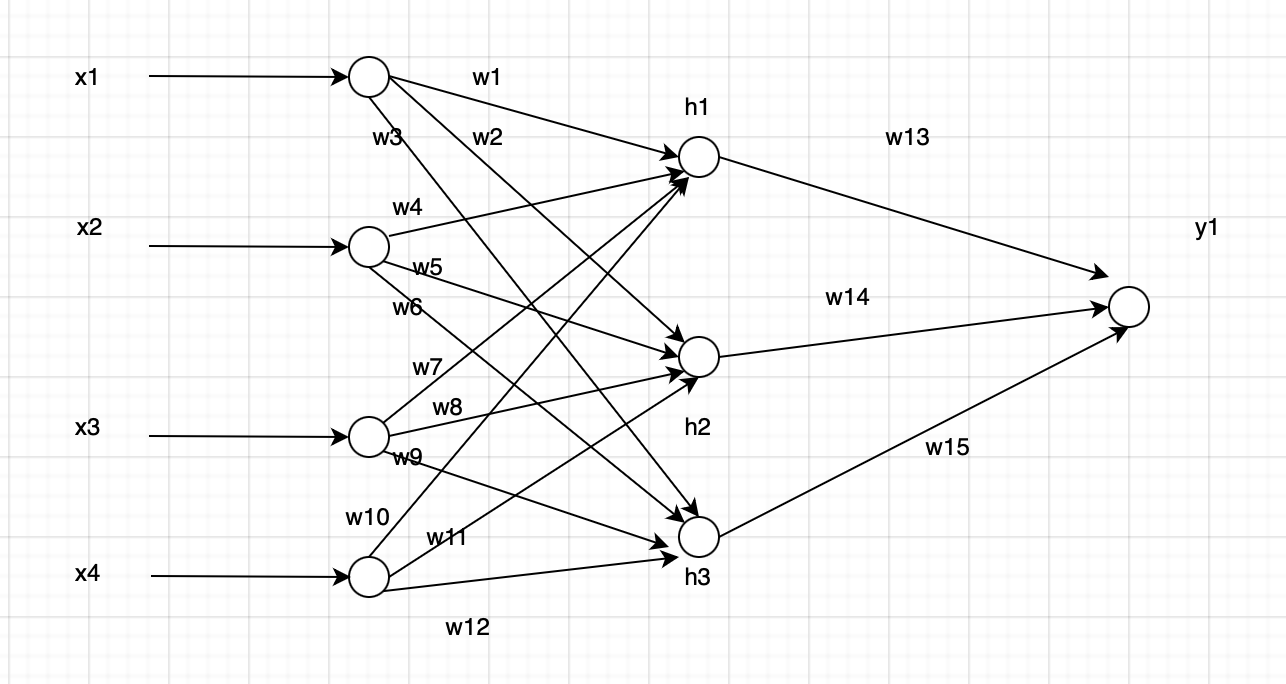
\includegraphics[width=0.8\linewidth]{fig/q41.png}
\caption{\label{fig:q41} \neural ANN Topology for All Features}
\end{figure}

\begin{figure}[H]
\centering
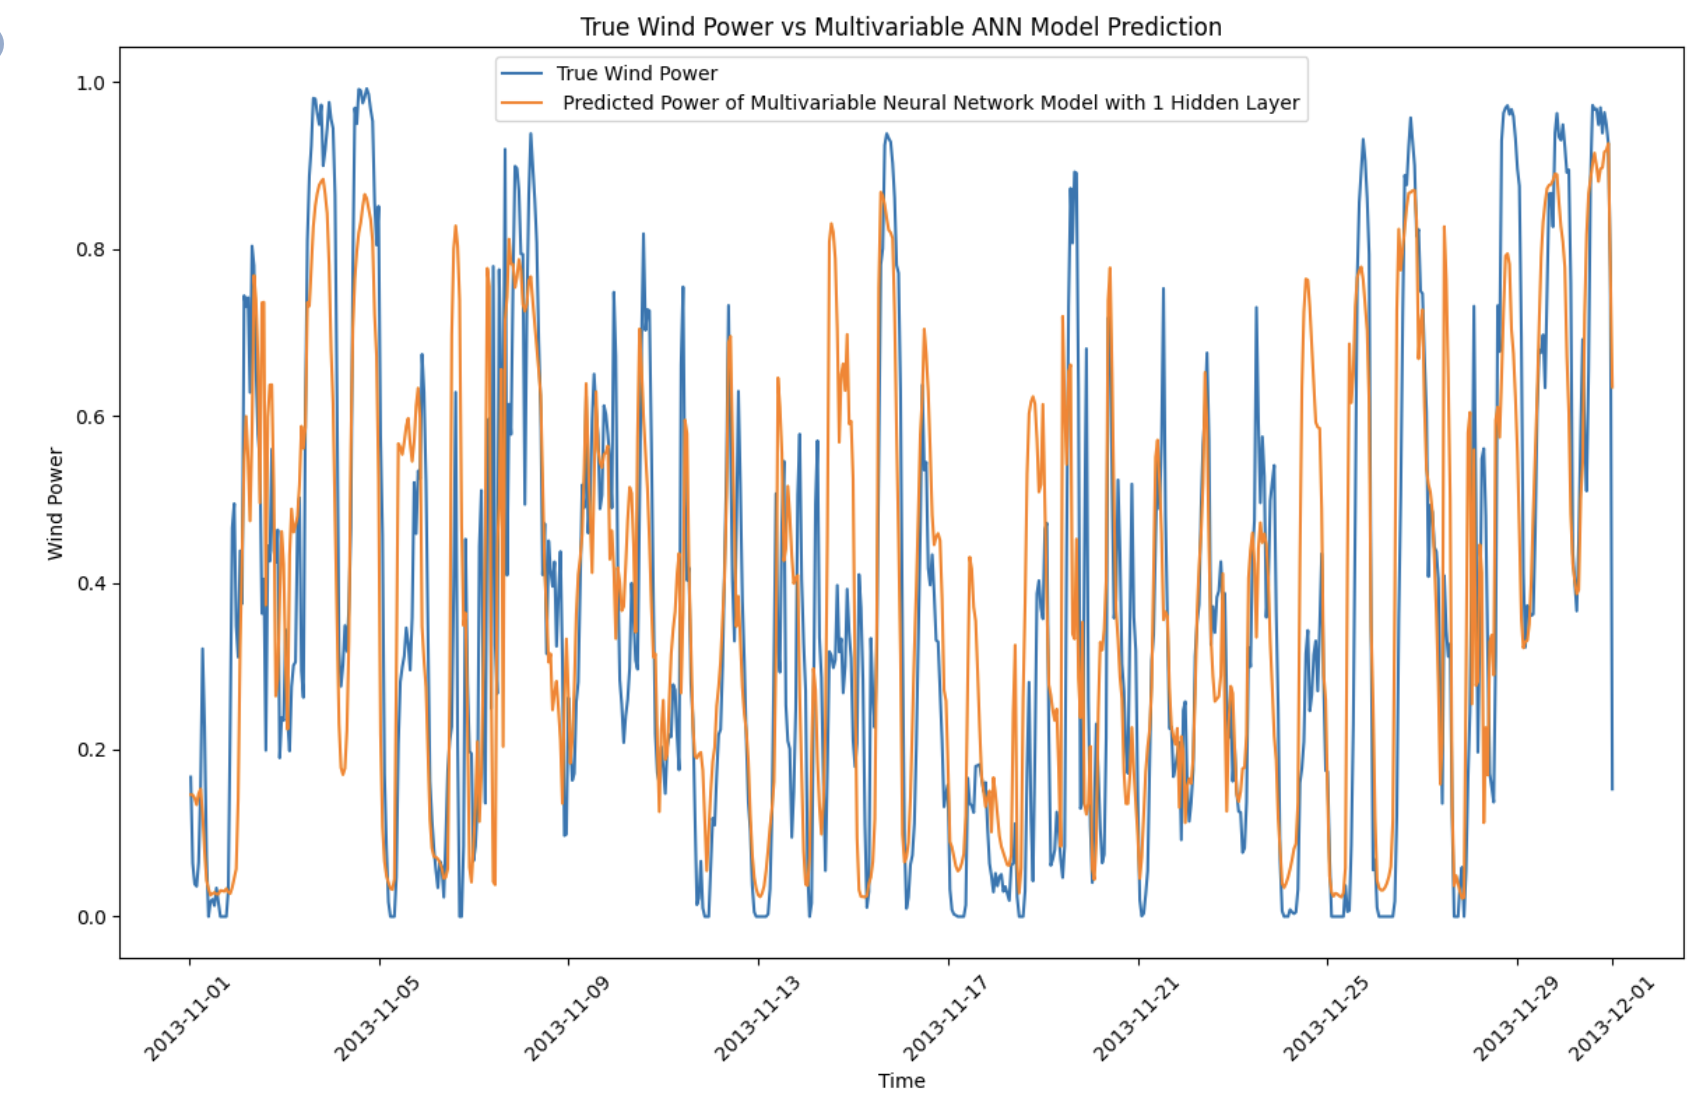
\includegraphics[width=1\linewidth]{fig/q42.png}
\caption{\label{fig:q42} Multi-variable ANN predicted power vs. actual measurement}
\end{figure}
RMSE for Multivariable ANN = 0.1928214148771009

}




\chapter*{reference}
{\url{http://https://amt.copernicus.org/articles/15/3465/2022/}}
% \bibitem[1]{https://amt.copernicus.org/articles/15/3465/2022/}


\end{document}

